% File mycontribution.tex to insert your text for your PRE6 contribution.
% Please rename the file when saving it. Give it the name of the first author!
% Put the pro12.sty style file in the same directory as your manuscript file
% for LATEX compilation.

\documentstyle[twoside,epsfig]{pro12}

% Some new commands for references
\newcommand{\JGR}[3]{\sl J. Geophys. Res.\rm, \bf #1\rm, #2, #3.}
\newcommand{\GRL}[3]{\sl Geophys. Res. Lett.\rm, \bf #1\rm, #2, #3.}
\newcommand{\NAT}[3]{\sl Nature\rm, \bf #1\rm, #2, #3.}
\newcommand{\PSS}[3]{\sl Planet. Space Sci.\rm, \bf #1\rm, #2, #3.}
\newcommand{\SCI}[3]{\sl Science\rm, \bf #1\rm, #2, #3.}
\newcommand{\ICAR}[3]{\sl Icarus\rm, \bf #1\rm, #2, #3.}
\newcommand{\SSR}[3]{\sl Space Sci. Rev.\rm, \bf #1\rm, #2, #3.}
\newcommand{\AJ}[3]{\sl Astrophys. J.\rm, \bf #1\rm, #2, #3.}
\newcommand{\AG}[3]{\sl Ann. Geophys.\rm, \bf #1\rm, #2, #3.}
\newcommand{\ASA}[3]{\sl Astron. Astrophys.\rm, \bf #1\rm, #2, #3.}


\head{T.H. Oswald et al.} {Numerical analysis of the SWAVES antennas}

\begin{document}

\title{
NUMERICAL ANALYSIS OF THE STEREO WAVES ANTENNAS: FIRST RESULTS}
\author{T.H. Oswald\adress{\sl  IWF/�AW, Austria}$\,$, W. Macher$^*$, G.Fischer$^*$, H.O. Rucker$^*$,J.L. Bougeret  \adress{\sl Observatoire de Paris-Meudon, France}, \\ M.L. Kaiser\adress{\sl NASA/GSFC, Greenbelt, MD, USA}, K. Goetz \adress{\sl University of Minnesota, USA}}

% Here the third author has the same affiliation as the second author.
% Emails addresses are not required, as we will make a separate email list of all
% participants at the end of the proceedings book (see PRE V book).

\maketitle

\begin{abstract}
% Enter the text of your abstract here
The SWAVES experiments onboard the two STEREO spacecraft will perform measurements of the non-thermal radio spectrum from 125 kHz up to about 16 MHz, observed from two different points at Earth orbit. For that purpose 3 orthogonal, six meter long monopole stacer antennas and a set of receivers are used, thereby enabling direction finding, i.e. the determination of the direction of arrival and the polarization state of the observed radio waves, in the lower part of the frequency range. Numerical wire-grid simulations of the antenna system are performed to determine the so-called effective length vectors of the antennas, which are the most suitable representation of the antenna properties in this context. The results of the first analysis are presented, with a view to the intended direction finding applications.
\end{abstract}

\section{Introduction}
\paragraph*{} One of the space missions, currently in the last phase of preparation is STEREO. STEREO is a space mission conducted by NASA to be launched in spring 2006. The mission consists of two space probes which will enter a heliocentric orbit. One spacecraft will orbit sun ahead of the earth, the other behind.

\paragraph*{} The scientific goal of the mission is to increase our knowledge of the physics of our solar system, especially:

\begin{itemize} \item Understanding the causes and mechanisms of CME initiation
\item Characterize the propagation of CMEs through the heliosphere
\item Discover the mechanism and sites of energetic particle acceleration in the low corona and the interplanetary medium
\item Develop a 3D time dependent model of the magnetic topology, temperature, density and velocity structure of the ambient solar wind
\end{itemize}

\paragraph*{} Among several other experiments, one particular important is STEREO WAVES (SWAVES). This experiment is designed to track interplanetary radio bursts and trace the generation and evolution of radio disturbances from the sun to earth orbit and beyond. Each spacecraft has three nearly orthogonal antennas. With this configuration it is possible to perform direction finding to find the direction of the origin of the received radiation and information about its polarization. When both spacecraft receive radiation from the same source at the same time, the actual location of the source can be pinpointed by the method of triangulation.

\paragraph*{} The technique of direction finding relies heavily upon the precise knowledge of the direction and the length of the three antennas. Unfortunately, the real behavior of the antennas is different than one would predict for the geometric configuration of the antennas. The reason is the perturbation of the body of the spacecraft. The surface of the body of the spacecraft is made of conducting material, so it can in principle be regarded as part of the antennas. As a result, each antenna behaves as if it would point into a slightly different direction with a slightly different length. The vector that describes the direction and length of this virtual antenna is called effective length vector. This effective length has to be determined before any direction finding can be conducted.

\section{Methods of calibration}
\paragraph*{}
There are three known methods to determine the effective length vectors of the antennas of a spacecraft: \begin{enumerate}
\item The numerical approach
\item The experimental approach (Rheometry)
\item In flight calibration
\end{enumerate}

\paragraph*{}
All three methods complement each other and are necessary components of the process of determination and validation of the antenna properties. We do the numerical and the experimental method at our institute. This paper is about the first results of the numerical method.

\paragraph*{}
The numerical method is realized by computer programs and consists of two steps. First, the distribution of the currents on the surface and the antennas is calculated, normally by using the method of moments (MoM). This distribution can be used to calculate the effective length vectors and other antenna properties, like antenna impedances, which is the second step.

\paragraph*{}
An analytical solution of the surface current distribution is normally impossible to find, owing to the complex structure of the spacecraft. This is the reason why one has to resort to numerical methods. For this purpose the surface of the spacecraft is modeled as a grid of wires with proper conductivities. The geometrical data and information about the material is fed into the software packages that do the actual calculation. The software package we use for the calculation of the current distribution is a modified version of the Antenna Scatterers Analysis Program (ASAP), an open source electromagnetic code written in Fortran77 and freely available in the internet. The output of this computation is a matrix, describing the surface current distribution. This data is, in turn, the input of the next stage of the calculation where the effective length vectors are computed. For this calculation we use the Matlab toolbox which was written at our institute.

\paragraph*{}
The computation has to be performed for all three antennas and for both spacecraft of the STEREO mission. Since the two spacecraft do not have the same shape, a separate wire grid model has to be constructed for each. The whole calculation will be done several times with a slightly different configuration, to investigate the influence of particular parts of the spacecraft on the deviation of the effective antenna axis from the geometrical axis. Fortunately, the effect of the frequency and direction of the incoming wave length vector on the effective length vectors is small at low frequencies where the antenna is short in relation to the wavelength. Additionally the imaginary part of the components of the effective length vectors vanishes. This is the frequency range, where the direction finding will be performed, thereby defining the constraint of the computation. This frequency range is called the quasistatic range.

\section{The spacecraft}
\paragraph*{}
The algorithm we used to compute the current distribution on the surface of the spacecraft imposed a limit on the minimum size of the structure details we could model. Features of the spacecraft we could include in our model where the hull, the two solar panels, the boom, the HGA dish, the low gain antennas and, of course, the SWAVES antennas, named E1, E2 and E3. Additionally we could model the rings that are mounted on the hull of the spacecraft (s/c). The rings were the only difference between the two spacecraft, we could model within the limitations of the algorithm. Spacecraft A has mounted one ring on the hull, while s/c B has a second one, mounted exactly on the opposite side. Our wiregrid model of s/c A can be seen on figure \ref{fig_sc}, the units of the axes are meters.


\begin{figure}[ht]
\begin{center}
\epsfig{file=spacecraft.eps,width=0.95\textwidth,angle=0}
\caption{The wiregrid model}
\label{fig_sc}
\end{center}
\end{figure}
% To put two figure-files next to each other use two \epsfig commands:
%\epsfig{file=figure2_1.eps,width=0.47\textwidth}
%\epsfig{file=figure2_2.eps,width=0.47\textwidth}
% by reducing the textwidth to <0.5; it is counted as one figure.


\paragraph*{}
The s/c fixed coordinate system is as shown in figure \ref{fig_sc}. Sun will normally be located on the side of the positive x axis, while the boom and the antennas point to the other side. The circumstance that the hull will often be between the source of the radiation and the antennas is also a reason why the antenna properties will be much influenced by the s/c structure. For the description of the antennas we use a polar coordinate system, where $\zeta$ is the angle from the positive x axis and $\xi$ is the azimuthal angle around the x axis. The azimuthal angle of E1 is defined to have $\xi=0^\circ$. E2 and E3 point to  $\xi=120^\circ$ and  $\xi=-120^\circ$ respectively. All three antennas have a colatitude of $\zeta= 125.26^\circ$.

\section{The computed effective length vectors}
\paragraph*{}
Figure \ref{fig_heff} shows the effective length vectors (in color) of s/c A at a frequency of 500kHz in relation to the physical antennas (in black), while table \ref{tab_heff} shows the results of both s/c in numerical form.

\begin{figure}[ht]
\begin{center}
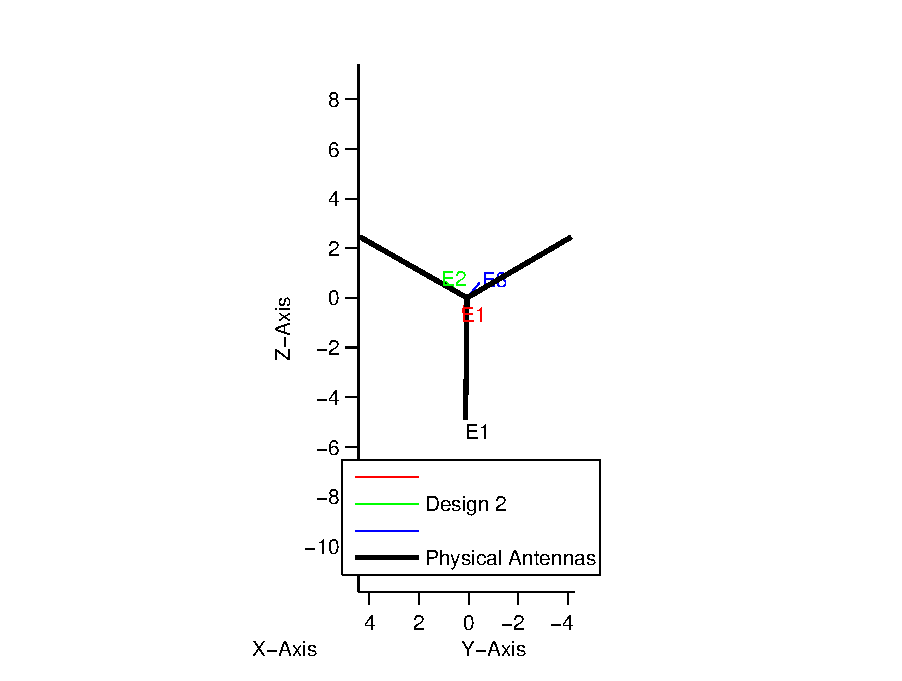
\epsfig{file=heff1.eps,width=0.45\textwidth,angle=0}
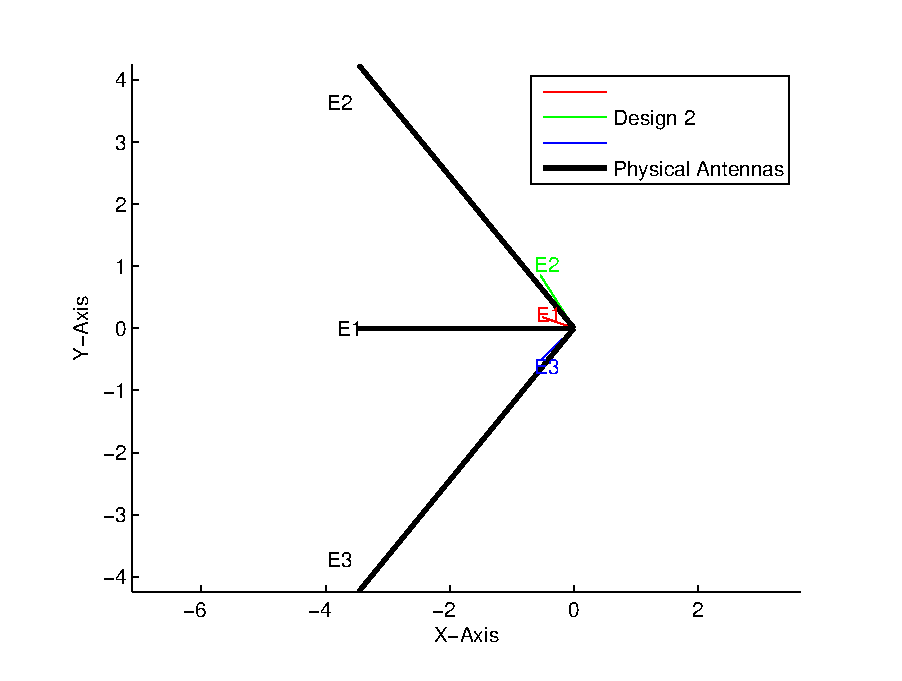
\epsfig{file=heff2.eps,width=0.45\textwidth,angle=0}
\caption{The effective length vectors}
\label{fig_heff}
\end{center}
\end{figure}



\begin{table}
\begin{center}
\label{tab_heff} \caption{Effective length vectors at 500kHz} \begin{tabular}{|c|c|c|c|c|} \hline  &  & Spacecraft A & Spacecraft B & Physical antennas \\ \hline E1 &  \begin{tabular}{c} \hline Length/m \\ \hline $\zeta/^\circ$ \\ \hline $\xi/^\circ$ \\ \hline \end{tabular} & \begin{tabular}{c} \hline  0.83\\ \hline  128.3\\ \hline  15.0\\ \hline \end{tabular} & \begin{tabular}{c} \hline  0.84\\ \hline  127.2\\ \hline  13.3\\ \hline \end{tabular} & \begin{tabular}{c} \hline 6.00 \\ \hline 125.26 \\ \hline 0.0 \\ \hline \end{tabular}  \\ \hline E2 & \begin{tabular}{c} \hline Length/m \\ \hline $\zeta/^\circ$ \\ \hline $\xi/^\circ$ \\ \hline \end{tabular} & \begin{tabular}{c} \hline  1.21\\ \hline  117.1\\ \hline  125.8\\ \hline \end{tabular} & \begin{tabular}{c} \hline  1.18\\ \hline  117.4\\ \hline  125.2\\ \hline \end{tabular} & \begin{tabular}{c} \hline 6.00 \\ \hline 125.26 \\ \hline 120.0 \\ \hline \end{tabular}  \\ \hline E3 &  \begin{tabular}{c} \hline Length/m \\ \hline $\zeta/^\circ$ \\ \hline $\xi/^\circ$ \\ \hline \end{tabular} & \begin{tabular}{c} \hline  0.99\\ \hline  123.5\\ \hline  -137.2\\ \hline \end{tabular} & \begin{tabular}{c} \hline  0.98\\ \hline  123.3\\ \hline  -135.4\\ \hline \end{tabular} & \begin{tabular}{c} \hline 6.00m \\ \hline 125.26� \\ \hline -120.0� \\ \hline \end{tabular}  \\ \hline \end{tabular}
\end{center}
\end {table}


\begin{figure}[ht]
\begin{center}
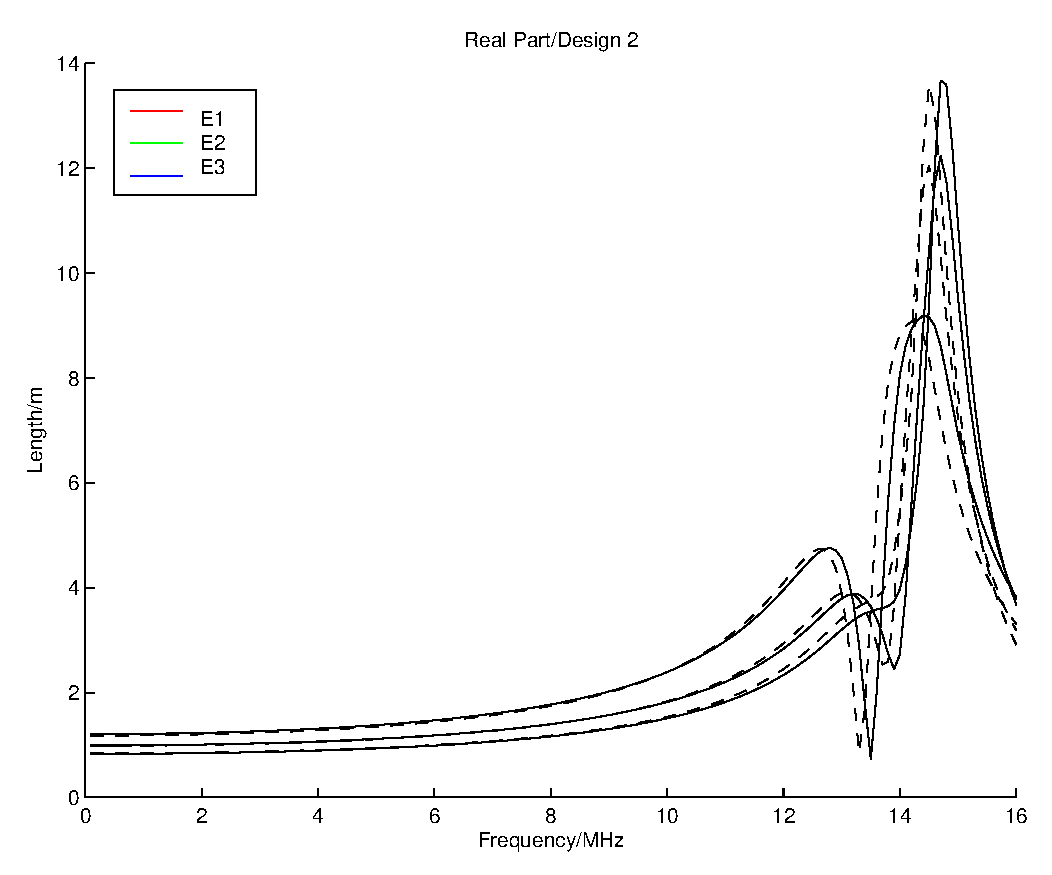
\epsfig{file=HeffReal.eps,width=0.45\textwidth,angle=0}
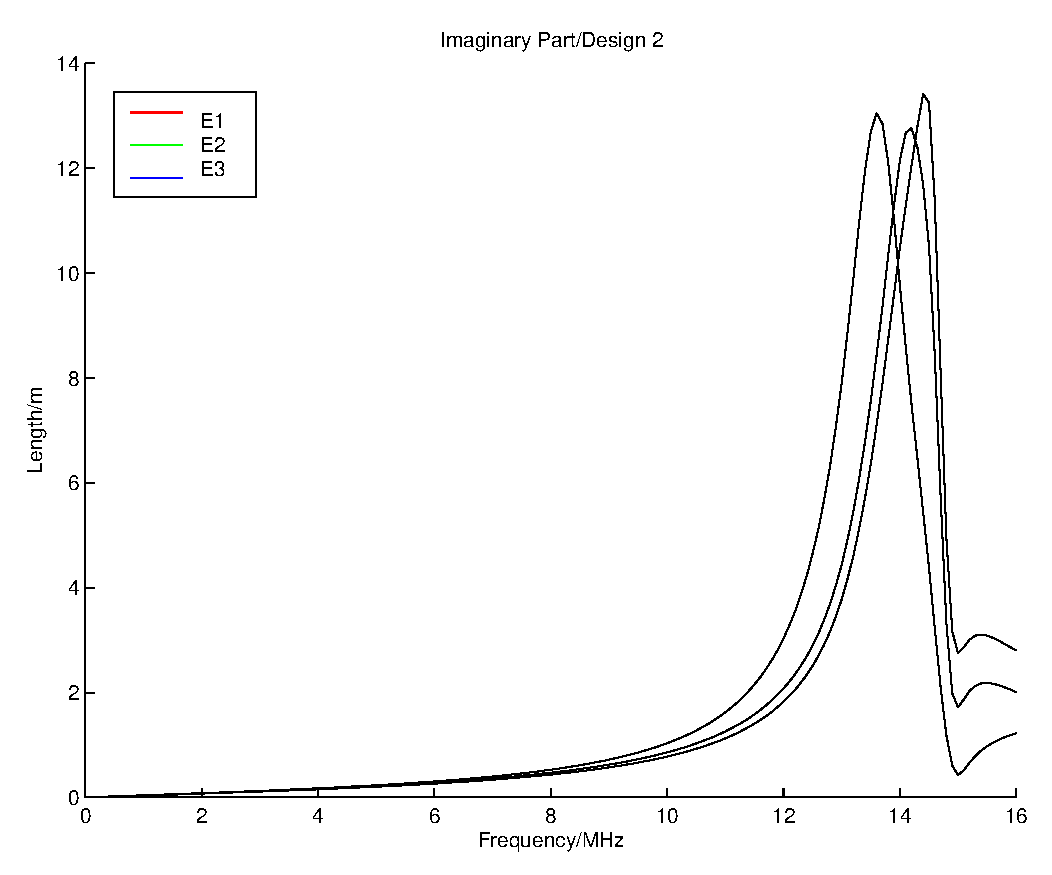
\epsfig{file=HeffImag.eps,width=0.45\textwidth,angle=0}
\caption{The real and imaginary parts of the effective length vectors}
\label{fig_heff2}
\end{center}
\end{figure}

\paragraph*{}
Figure \ref{fig_heff2} shows the real and imaginary parts of the electric antennas as a function of frequency. We computed them for a frequency range from 100kHz to 16MHz. One can see a number of features at those plots. The real part behaves almost constant at a low frequency, while the imaginary part approaches zero as the frequency becomes small. The opposite behavior can be seen near the first resonance frequency. There the effective length vectors become erratic. Direction finding is not possible at this frequency range.

\begin{figure}[ht]
\begin{center}
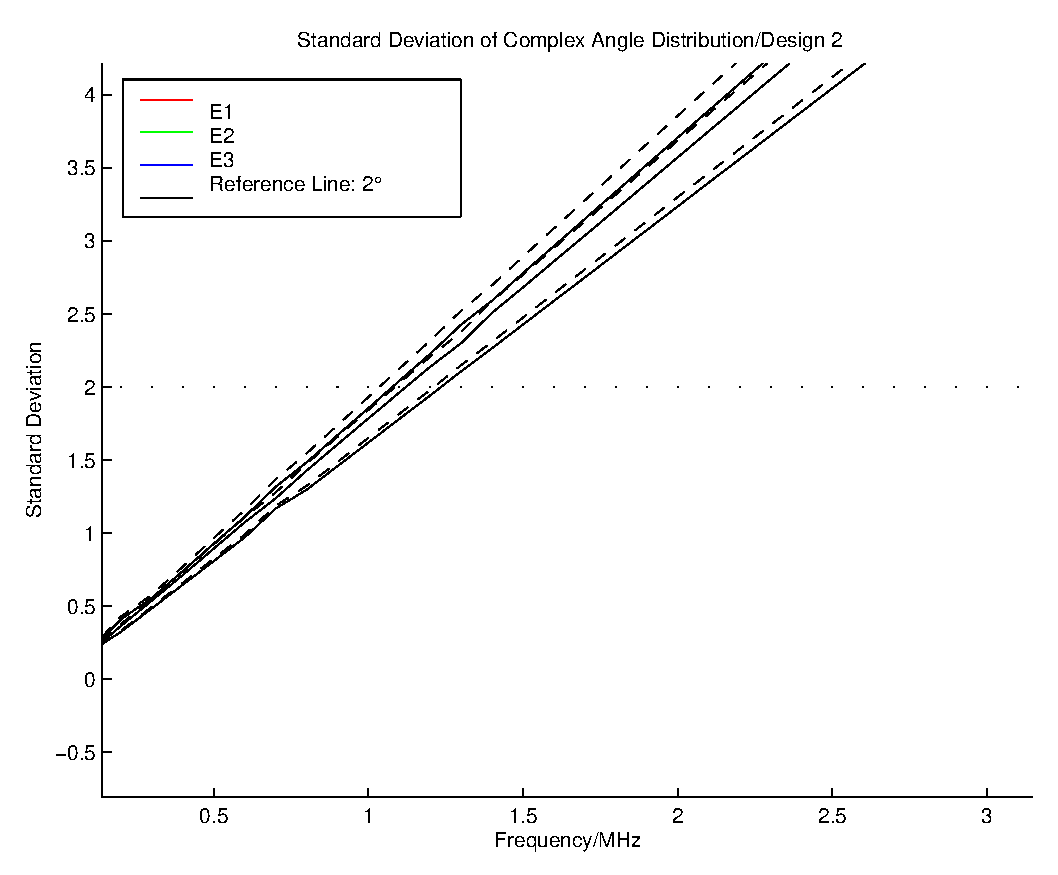
\epsfig{file=std1.eps,width=0.80\textwidth,angle=0}
\caption{The standard deviation of the length of the effective length vectors}
\label{fig_std1}
\end{center}
\end{figure}
\begin{figure}[ht]
\begin{center}
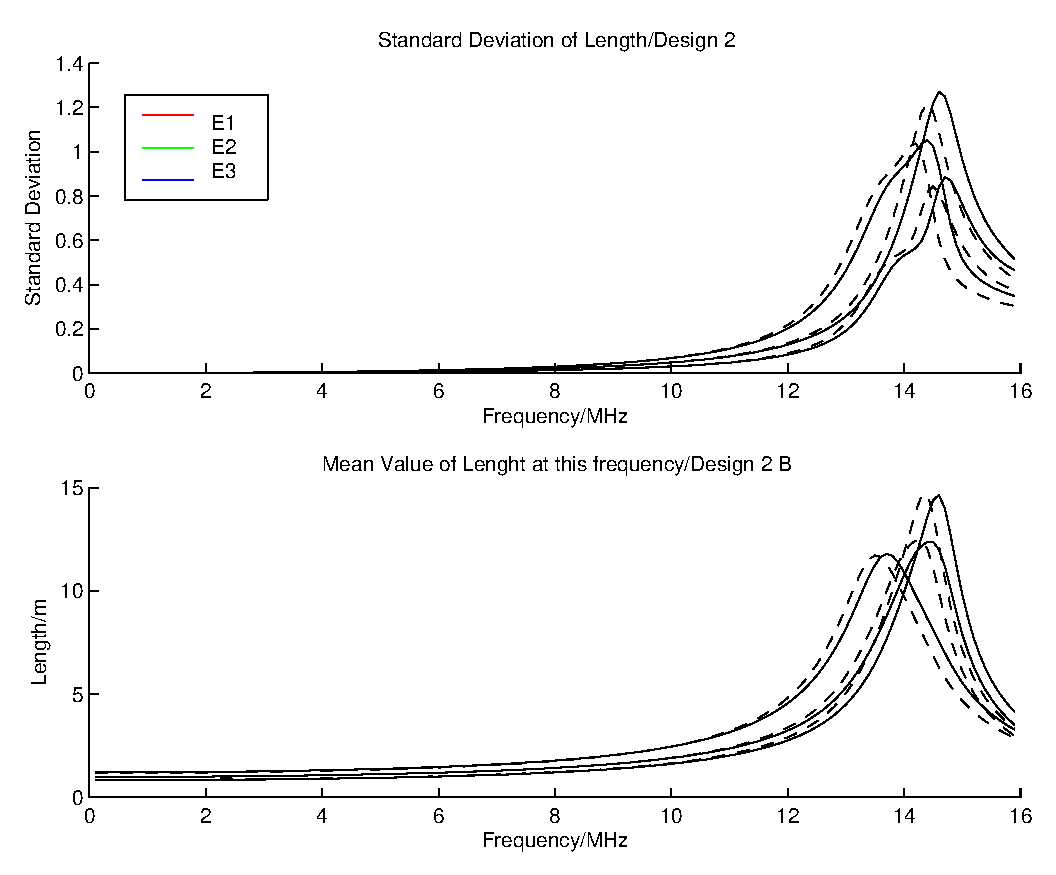
\epsfig{file=std2.eps,width=0.80\textwidth,angle=0}
\caption{The standard deviation of the direction of the effective length vectors}
\label{fig_std2}
\end{center}
\end{figure}
\section{The variation of the effective length vector due to the direction of incidence}
\paragraph*{}
As we mentioned before, the effective length vector of an antenna depends on the direction of the incoming wave. We tried to quantify this by using statistical methods. We treated the direction of incidence as a random parameter and calculated the standard deviation of the length and direction of the electric antennas as a function of frequency. The results are shown in figures \ref{fig_std1} and \ref{fig_std2}. As one can see, the variation of the length is very small and seems to be of no concern. This is not true for the direction of the electric antennas. We normally consider direction finding as possible as long as the direction of the effective length vectors is known to an accuracy of 2 degrees. As one can see on the plot, according to our estimation, this boundary would be reached at a frequency of only a little bit more than 1MHz.

\section{The impedance}
\paragraph*{}
We also computed the input impedances of the antennas. As an example, the impedances of the antennas of s/c A are shown in figures \ref{fig_imps1} and \ref{fig_imps2}.
\begin{figure}[ht]
\begin{center}
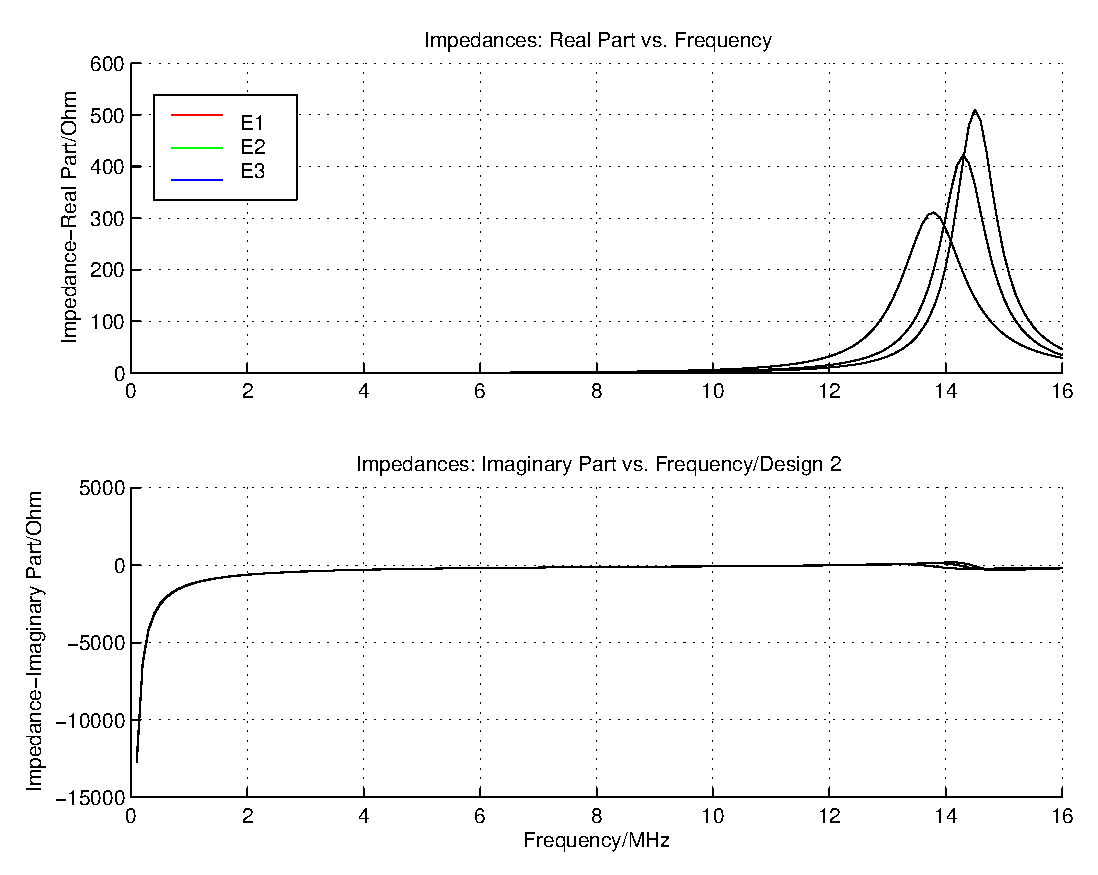
\epsfig{file=imps1.eps,width=0.80\textwidth,angle=0}
\caption{The standard deviation of length and direction of the effective length vectors}
\label{fig_imps1}
\end{center}
\end{figure}

\begin{figure}[ht]
\begin{center}
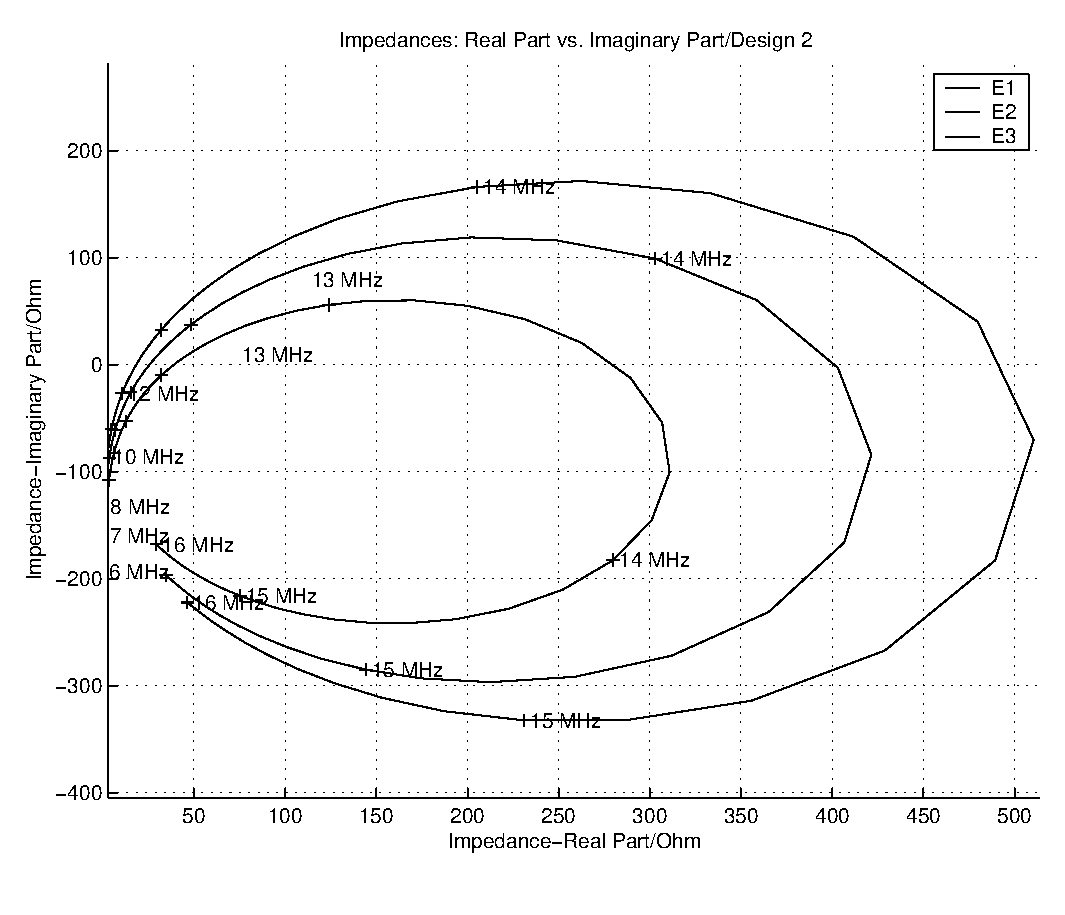
\epsfig{file=imps2.eps,width=0.80\textwidth,angle=0}
\caption{The standard deviation of length and direction of the effective length vectors}
\label{fig_imps2}
\end{center}
\end{figure}

\section{Conclusion}
\paragraph*{}
We showed that the effective length vectors that represent the receiving and transmitting properties of the antennas, differ substantially from the physical ones. Therefore antenna calibration is absolutely necessary when we want to perform direction finding. We presented the first results from the numerical computation and showed that the variation due to different directions of the incident waves are expected to be a limiting factor.

\paragraph*{}
Our next steps will be the experimental determination of the effective length vectors and the the use of better electromagnetic code, so that we can model the s/c structure to a higher accuracy.


\section*{References}
\everypar={\hangindent=1truecm \hangafter=1}

% Use the references.tex file to look for commonly used
% planetary radio science references, and then simply copy and
% paste it. Our reference list is quite long, in case you
% don't find the reference, please write it in the same way
% as given the example references below.

Cecconi, B., and P. Zarka, Direction finding and antenna
calibration through analytical inversion of radio measurements
performed using a system of 2 or 3 electric dipole wire antennas,
{\sl Radio Science}, submitted, 2004.

Fainberg, J., Technique to determine location of radio sources
from measurements taken on spinning spacecraft, NASA Technical
Memorandum 80598, 1979.

Fainberg, J., Technique to determine location of radio sources from
measurements taken on spinning spacecraft. NASA,
{\sl Technical Memorandum} {\bf 80598}, 1979.

Fischer, G., W. Macher, H. O. Rucker, H. P. Ladreiter, D. F. Vogl,
and the Cassini RPWS Team,  Wire-Grid modeling of Cassini
spacecraft for the determination of effective antenna length
vectors of the RPWS antennas, in {\sl Planetary Radio Emissions
V}, edited by H. O. Rucker, M. L. Kaiser, and Y. Leblanc, Austrian
Academy of Sciences Press, Vienna, 347--356, 2001.

Ladreiter, H. P., A. Lecacheux, W. Macher, and H. O. Rucker, Radio
wave direction finding on Cassini, Publ. Austrian Academy of
Sciences, Space Research Institute, {\bf 95}, Graz, 1994.

Ladreiter, H. P., P. Zarka, A. Lecacheux, W. Macher, H. O. Rucker,
R. Manning, D. A. Gurnett, and W. S. Kurth,
Analysis of electromagnetic wave direction finding performed by
spaceborne antennas using singular value decomposition techniques,
{\sl Radio Sci.,} {\bf 30,} 1699--1712, 1995.

Ladreiter, H. P., P. Zarka, A. Lecacheux, W. Macher, H. O. Rucker,
R. Manning, D. A. Gurnett, and W. S. Kurth, Analysis of
electromagnetic wave direction finding performed by spaceborne
antennas using singular--value decomposition techniques, {\sl
Radio Science}, {\bf 30}, 1699, 1995.

Lecacheux, A., Direction Finding of a Radiosource of Unknown
Polarization with Short Electric Antennas on a Spacecraft, {\sl
Astron. Astrophys.}, {\bf 70}, 701, 1978.

Manning, R., and J. Fainberg, A new method of measuring radio
source parameters of a partially polarized distributed source from
spacecraft observations, {\sl Space Sci.\ Instrum.,} {\bf 5,} 161, 1980.

Macher, W., Theorie effektiver H\"ohenvektoren von Antennen mit
Anwendung auf das Radio and Plasma Wave Science Experiment der
Cassini Raumsonde, Diploma Thesis at the University of Technology
Graz, Austria, 1997.

Oswald T.H., W. Macher, G.Fischer, H.O. Rucker, First results of STEREO/WAVES Antenna calibration, Technical Report of the Space Research Institute/Austrian Academy of Science, 2004

Rucker, H. O., W. Macher, and S. Albrecht, Experimental and
Theoretical Investigations on the Cassini RPWS Antennas, in {\it
Planetary Radio Emissions IV}, edited by H. O. Rucker, S. J.
Bauer, and A. Lecacheux, Austrian Academy of Sciences Press,
Vienna, 327--337, 1997.

Rucker, H. O., W. Macher, R. Manning, and H. P. Ladreiter, Cassini
model rheometry, {\it Radio Science}, {\bf 31}, 6, 1299--1311,
1996.

Rucker, H. O., W. Macher, R. Manning, and H.~P. Ladreiter,
Cassini model rheometry, {\sl Radio Sci.,} {\bf 31,} 1299--1311, 1996.

Vogl, D. F., H. P. Ladreiter, P. Zarka, H. O. Rucker, W. Macher,
W. S. Kurth, D. A. Gurnett, and G. Fischer, First results on the
calibration of the Cassini RPWS antenna system, in {\it Planetary
Radio Emissions V}, edited by H. O. Rucker, M. L. Kaiser, and Y.
Leblanc, Austrian Academy of Sciences Press, Vienna, 357--365,
2001.


\end{document}

